\newpage
\section{Classe \Iclass{triangle}} % (fold)
\label{sec:classe_triangle}

\subsection{Attributes of a triangle} % (fold)
\label{sub:attributes_of_a_triangle}
The triangle object is created using the \Imeth{triangle}{new} method, for example with
\begin{mybox}
   Creation  | T.ABC = triangle : new ( z.A , z.B , z.C ) |
\end{mybox}
(See examples:  \ref{sub:alternate}; \ref{sub:apollonius_circle}; \ref{sub:excircles} ). Multiple attributes are then created.

\bgroup
\catcode`_=12
\small
\captionof{table}{Triangle attributes.}\label{triangle:att}
\begin{tabular}{ll}
\toprule
\textbf{Attributes}     & \textbf{Application}\\
\Iattr{triangle}{pa} &T.ABC.pa \\
\Iattr{triangle}{pb} &T.ABC.pb \\
\Iattr{triangle}{pc} &T.ABC.pc \\
\Iattr{triangle}{type} & 'triangle' \\
\Iattr{triangle}{circumcenter} & T.ABC.circumcenter\\
\Iattr{triangle}{centroid} &T.ABC.centroid\\
\Iattr{triangle}{incenter} &T.ABC.incenter\\
\Iattr{triangle}{orthocenter}  &T.ABC.orthocenter\\
\Iattr{triangle}{eulercenter} &T.ABC.eulercenter  \\
\Iattr{triangle}{spiekercenter} &T.ABC.spiekercenter  \\
\Iattr{triangle}{a}& It's the length of the side opposite the first vertex  \\
\Iattr{triangle}{b}& It's the length of the side opposite the second verte\\
\Iattr{triangle}{c}& It's the length of the side opposite the third vertex \\
\Iattr{triangle}{alpha}& Vertex angle of the first vertex\\
\Iattr{triangle}{beta}& Vertex angle of the second vertex\\
\Iattr{triangle}{gamma}& Vertex angle of the third vertex\\
\Iattr{triangle}{ab}& Line defined by the first two points of the triangle\\
\Iattr{triangle}{bc}& Line defined by the last two points \\
\Iattr{triangle}{ca}&  Line defined by the last and the first points of the triangle\\
\bottomrule %
\end{tabular}
\egroup

\subsection{Triangle attributes: angles} % (fold)
\label{sub:triangle_attributes_angles}

\begin{minipage}{.6\textwidth}
\begin{verbatim}
\begin{tkzelements}
  z.A       = point: new(0,0)
  z.B       = point: new(5,0)
  z.C       = point: new(2,3)
  T.ABC     = triangle: new (z.A,z.B,z.C)
\end{tkzelements}
\def\wangle#1{\tkzDN[2]{%
  \tkzUseLua{math.deg(T.ABC.#1)}}}
\begin{tikzpicture}
\tkzGetNodes
  \tkzDrawPolygons(A,B,C)
  \tkzLabelAngle(B,A,C){$\wangle{alpha}^\circ$}
  \tkzLabelAngle(C,B,A){$\wangle{beta}^\circ$}
  \tkzLabelAngle(A,C,B){$\wangle{gamma}^\circ$}
\end{tikzpicture}
\end{verbatim}
\end{minipage}
\begin{minipage}{.4\textwidth}
\begin{tkzelements}
   z.A       = point: new(0,0)
   z.B       = point: new(5,0)
   z.C       = point: new(2,3)
   T.ABC     = triangle: new (z.A,z.B,z.C)
\end{tkzelements}
\def\wangle#1{\tkzDN[2]{\tkzUseLua{math.deg(T.ABC.#1)}}}
\begin{tikzpicture}
\tkzGetNodes
\tkzDrawPolygons(A,B,C)
\tkzLabelAngle(B,A,C){$\wangle{alpha}^\circ$}
\tkzLabelAngle(C,B,A){$\wangle{beta}^\circ$}
\tkzLabelAngle(A,C,B){$\wangle{gamma}^\circ$}
\end{tikzpicture}
\end{minipage}
% subsection triangle_attributes_angles (end)

\subsubsection{Example: triangle attributes} % (fold)
\label{ssub:example_triangle_attributes}
\begin{minipage}{.5\textwidth}
   \begin{verbatim}
   \begin{tkzelements}
      z.a   = point: new (0 , 0)
      z.b   = point: new (4 , 0)
      z.c   = point: new (0 , 3)
      T.abc = triangle : new (z.a,z.b,z.c)
      z.O   = T.abc.circumcenter
      z.I   = T.abc.incenter
      z.H   = T.abc.orthocenter
      z.G   = T.abc.centroid
      a     = T.abc.a
      b     = T.abc.b
      c     = T.abc.c
      alpha =  T.abc.alpha
      beta  =  T.abc.beta
      gamma =  T.abc.gamma
   \end{tkzelements}
   \begin{tikzpicture}
      \tkzGetNodes
      \tkzDrawPolygon(a,b,c)
      \tkzDrawPoints(a,b,c,O,G,I,H)
      \tkzLabelPoints(a,b,c,O,G,I)
      \tkzLabelPoints[above right](H)
      \tkzDrawCircles(O,a)
      \tkzLabelSegment[sloped](a,b){\tkzUseLua{c}}
      \tkzLabelSegment[sloped,above](b,c){\tkzUseLua{a}}
   \end{tikzpicture}
   \end{verbatim}
\end{minipage}
\begin{minipage}{.5\textwidth}
\begin{tkzelements}
   scale = 1.2
   z.a = point: new (0 , 0)
   z.b = point: new (4 , 0)
   z.c = point: new (0 , 3)
   T.abc = triangle : new (z.a,z.b,z.c)
   z.O = T.abc.circumcenter
   z.I = T.abc.incenter
   z.H = T.abc.orthocenter
   z.G = T.abc.centroid
   a = T.abc.a
   b = T.abc.b
   c = T.abc.c
   alpha =  T.abc.alpha
   beta  =  T.abc.beta
   gamma =  T.abc.gamma
\end{tkzelements}
\hspace*{\fill}
\begin{tikzpicture}
\tkzGetNodes
\tkzDrawPolygon(a,b,c)
\tkzDrawPoints(a,b,c,O,G,I,H)
\tkzLabelPoints(a,b,c,O,G,I)
\tkzLabelPoints[above right](H)
\tkzDrawCircles(O,a)
\tkzLabelSegment[sloped](a,b){\tkzUseLua{c}}
\tkzLabelSegment[sloped,above](b,c){\tkzUseLua{a}}
\end{tikzpicture}
\end{minipage}

% subsubsection example_triangle_attributes (end)

% subsection attributes_of_a_triangle (end)

\subsection{Methods of the class triangle} % (fold)
\label{sub:methods_of_the_class_triangle}

\bgroup
\catcode`_=12
\small
\begin{minipage}{\textwidth}
\captionof{table}{triangle methods.}\label{triangle:met}
\begin{tabular}{ll}
\toprule
\textbf{Methods} & \textbf{Comments}     \\
\midrule
\Imeth{triangle}{new} (a, b ,c) & |T.ABC = triangle : new (z.A,z.B,z.C)|    \\
 ... & |T| or |T.name| with what you want for name, is possible.\\
\midrule 
 \textbf{Points} &\\
\midrule 
\Imeth{triangle}{lemoine\_point ()} &  |T.ABC : lemoine_point ()| intersection os the symmedians\\
\Imeth{triangle}{symmedian\_point ()}  & Lemoine point  or the Grebe point \\
\Imeth{triangle}{bevan\_point ()}  &  Circumcenter of the excentral triangle\\
\Imeth{triangle}{mittenpunkt\_point ()}  &  Symmedian point of the excentral triangle\\
\Imeth{triangle}{gergonne\_point ()}  & Intersection of the three cevians that lead to the contact points \\
\Imeth{triangle}{nagel\_point () } & Intersection of the three cevians that lead to the extouch points\\
\Imeth{triangle}{feuerbach\_point () } & The point at which the incircle and euler circle are tangent. \\
\Imeth{triangle}{spieker\_center ()} &  Incenter of the medial triangle \\
\Imeth{triangle}{barycenter (ka,kb,kc)} & |T.ABC: barycenter (2,1,1)| barycenter of |({A,2},{B,1},{C,1}) |\\
\Imeth{triangle}{base (u,v)  }  &  |z.D = T.ABC: base(1,1)| \tkzar ABDC is a parallelogram   \\
\Imeth{triangle}{projection (p) }   &  Projection of a point on the sides \\
\Imeth{triangle}{euler\_points () } & Euler points of euler circle   \\
\Imeth{triangle}{nine\_points () }   & 9 Points of the euler circle  \\
\Imeth{triangle}{parallelogram ()} & |z.D = T.ABC : parallelogram ()| \tkzar ABCD is a parallelogram\\
\midrule
 \textbf{Lines} &\\
\midrule 
\Imeth{triangle}{altitude (n) }  & |L.AHa = T.ABC : altitude () | n empty or 0  line from $A$  
\footnote{|z.Ha = L.AHa.pb| recovers the common point of the opposite side and altitude. The method |orthic| is usefull.}\\
\Imeth{triangle}{bisector (n) }  & |L.Bb = T.ABC : bisector (1) |  n = 1   line from $B$     \footnote{|_,z.b = get_points(L.Bb)| recovers the common point of the opposite side and bisector. }\\
\Imeth{triangle}{bisector\_ext(n) }   &   n=2  line from the third vertex.\\
\Imeth{triangle}{symmedian\_line (n)}  & Cevian with respect to Lemoine point. \\
\Imeth{triangle}{euler\_line () } & the line through $N$ ,$G$, $H$ and $O$ if the triangle is not equilateral
\footnote{N center of nine points circle, G centroid, H orthocenter , O circum center } \\
\Imeth{triangle}{antiparallel(pt,n)} & n=0 antiparallel through pt to $(BC)$, n=1 to $(AC)$ etc.\\
\midrule 
 \textbf{Circles} &\\
\midrule 
\Imeth{triangle}{euler\_circle ()} & C.|NP = T.ABC : euler_circle ()| \tkzar $N$ euler point 
 \footnote{ The midpoint of each side of the triangle, the foot of each altitude, the midpoint of the line segment from each vertex of the triangle to the orthocenter.}   \\
\Imeth{triangle}{circum\_circle ()}  & |C.OA = T.ABC : circum ()| Triangle's circumscribed circle \\
\Imeth{triangle}{in\_circle ()}   &   Inscribed circle of  the triangle\\
\Imeth{triangle}{ex\_circle (n)}  &  Circle tangent to  the three sides of the triangle ; n =1 swap ; n=2 2 swap \\
\Imeth{triangle}{first\_lemoine\_circle ()}  & The center is the midpoint between Lemoine point and the circumcenter.\footnote{
Through the Lemoine point draw lines parallel to the triangle's sides. The points where the parallel lines intersect the sides of ABC
 then lie on a circle known as the first Lemoine circle. } \\
\Imeth{triangle}{second\_lemoine\_circle ()} & see example \ref{sub:antiparallel_through_lemoine_point}\\
\Imeth{triangle}{spieker\_circle ()} & The incircle of the medial triangle\\

\bottomrule
\end{tabular}
\end{minipage}
\egroup

Remark: If you don't need to use the triangle object several times, you can obtain a bisector or a altitude with the next functions 

|bisector (z.A,z.B,z.C)| and |altitude (z.A,z.B,z.C)| See (\ref{misc})

\clearpage\newpage
\bgroup
\catcode`_=12
\small
\begin{minipage}{\textwidth}
\begin{center}
%\caption{Methods of the class triangle (follow-up) }
\begin{tabular}{ll}
\toprule
\textbf{Methods} & \textbf{Comments}     \\
\midrule 
 \textbf{Triangles} &\\
\midrule 
\Imeth{triangle}{orthic ()}  &  |T = T.ABC : orthic ()| triangle joining the feet of the altitudes   \\
\Imeth{triangle}{medial ()}  &   |T = T.ABC : medial ()| triangle with vertices at the midpoints\\
\Imeth{triangle}{incentral ()}    &   Cevian triangle of the triangle with respect to its incenter \\
\Imeth{triangle}{excentral ()  }  &   Triangle with vertices corresponding to the excenters   \\
\Imeth{triangle}{extouch ()}  & Triangle formed by the points of tangency with the excircles    \\
\Imeth{triangle}{intouch () } &  Contact triangle formed by the points of tangency of the incircle \\
\Imeth{triangle}{tangential ()} & Triangle formed by the lines tangent to the circumcircle at the vertices\\
\Imeth{triangle}{feuerbach ()} & Triangle formed by the points of tangency of the euler circle with the excircles\\
\Imeth{triangle}{anti () }&  Anticomplementary Triangle The given triangle is its medial triangle.   \\
\Imeth{triangle}{cevian (pt)} & Triangle formed with the endpoints of the three cevians with respect to |pt|.\\
\Imeth{triangle}{symmedian ()} & Triangle formed with the intersection points of the symmedians. \\
\Imeth{triangle}{euler ()} &  Triangle formed with the euler points \\
\midrule 
\midrule 
 \textbf{Miscellaneous} &\\
\midrule 
\Imeth{triangle}{area ()}   & $ \mathcal{A}$| = T.ABC: area ()|\\
\Imeth{triangle}{barycentric\_coordinates (pt)} & Triples of numbers corresponding to masses placed at the vertices\\
\Imeth{triangle}{in\_out (pt)}  & Boolean. Test if |pt| is inside the triangle\\
\Imeth{triangle}{check\_equilateral ()} & Boolean. Test if the triangle is equilateral\\
\bottomrule
\end{tabular}
\end{center}
\end{minipage}
\egroup
% subsubsection methods_of_the_class_triangle (end)

\subsubsection{Euler line} % (fold)
\label{ssub:euler_line}

\begin{minipage}{.5\textwidth}
\begin{tkzexample}[latex=0cm,small,code only]
\begin{tkzelements}
   z.A           = point: new (0 , 0)
   z.B           = point: new (6 , 0)
   z.C           = point: new (1.5 , 3.5)
   T.ABC         = triangle: new (z.A,z.B,z.C)
   z.O           = T.ABC.circumcenter
   z.G           = T.ABC.centroid
   z.N           = T.ABC.eulercenter
   z.H           = T.ABC.orthocenter
   z.P,z.Q,z.R   = get_points (T.ABC: orthic())
   z.K,z.I,z.J   = get_points (T.ABC: medial ())
\end{tkzelements}
\begin{tikzpicture}
   \tkzGetNodes
   \tkzDrawLines[blue](O,H)
   \tkzDrawCircle[red](N,I)
   \tkzDrawCircles[teal](O,A)
   \tkzDrawSegments(A,P B,Q C,R)
   \tkzDrawSegments[red](A,I B,J C,K)
   \tkzDrawPolygons(A,B,C)
   \tkzDrawPoints(A,B,C,N,I,J,K,O,P,Q,R,H,G)
   \tkzLabelPoints(A,B,C,I,J,K,P,Q,R,H)
   \tkzLabelPoints[below](N,O,G)
\end{tikzpicture}
\end{tkzexample}
\end{minipage}
\begin{minipage}{.5\textwidth}
\begin{tkzelements}
 z.A    = point: new (0 , 0)
 z.B    = point: new (6 , 0)
 z.C    = point: new (1.5 , 3.5)
 T.ABC  = triangle: new (z.A,z.B,z.C)
 z.O    = T.ABC.circumcenter
 z.G    = T.ABC.centroid
 z.N    = T.ABC. eulercenter
 z.H    = T.ABC. orthocenter
 z.P,z.Q,z.R    = get_points (T.ABC: orthic())
 z.K,z.I,z.J    = get_points (T.ABC: medial ())
\end{tkzelements}
\hspace*{\fill}
\begin{tikzpicture}
\tkzGetNodes
\tkzDrawLines[blue](O,H)
\tkzDrawCircle[red](N,I)
\tkzDrawCircles[teal](O,A)
\tkzDrawSegments(A,P B,Q C,R)
\tkzDrawSegments[red](A,I B,J C,K)
\tkzDrawPolygons(A,B,C)
\tkzDrawPoints(A,B,C,N,I,J,K,O,P,Q,R,H,G)
\tkzLabelPoints(A,B,C,I,J,K,P,Q,R)
\tkzLabelPoints[below](N,O,G,H)
\end{tikzpicture}
\end{minipage}

%\caption{Euler line}
% subsubsection euler_line (end)

\subsection{Harmonic division and bisector} % (fold)
\label{sub:harmonic_division_and_bisector}

\begin{minipage}{.4\textwidth}
   \begin{verbatim}
   \begin{tkzelements}  
      scale    =  .4
      z.A      = point: new (0 , 0)
      z.B      = point: new (6 , 0)
      z.M      = point: new (5 , 4)
      T.AMB    = triangle : new (z.A,z.M,z.B)
      L.AB     = T.AMB.ca
      L.bis    = T.AMB : bisector (1)
      z.C      = L.bis.pb
      L.bisext = T.AMB : bisector_ext (1)
      z.D      = intersection (L.bisext,L.AB)
      L.CD     = line: new (z.C,z.D)
      z.O      = L.CD.mid
      L.AM     = line: new (z.A,z.M)
      L.LL     = L.AM : ll_from (z.B)
      L.MC     = line: new (z.M,z.C)
      L.MD     = line: new (z.M,z.D)
      z.E      = intersection (L.LL,L.MC)
      z.F      = intersection (L.LL,L.MD)
   \end{tkzelements}
   \end{verbatim}
\end{minipage}
\begin{minipage}{.6\textwidth}
\begin{tkzelements}  
   scale =.4
   z.A  = point: new (0 , 0)
   z.B  = point: new (6 , 0)
   z.M  = point: new (5 , 4)
   T.AMB    = triangle : new (z.A,z.M,z.B)
   L.AB = T.AMB.ca
   L.bis    = T.AMB : bisector (1)
   z.C  = L.bis.pb
   L.bisext = T.AMB : bisector_ext (1)
   z.D  = intersection (L.bisext,L.AB)
   L.CD = line: new (z.C,z.D)
   z.O  = L.CD.mid
   L.AM = line: new (z.A,z.M)
   L.LL = L.AM : ll_from (z.B)
   L.MC = line: new (z.M,z.C)
   L.MD = line: new (z.M,z.D)
   z.E  = intersection (L.LL,L.MC)
   z.F  = intersection (L.LL,L.MD)
\end{tkzelements}
\hspace{\fill}   
\begin{tikzpicture}
  \tkzGetNodes
  \tkzDrawPolygon(A,B,M)
  \tkzDrawCircle[purple](O,C)
  \tkzDrawSegments[purple](M,E M,D E,F)
  \tkzDrawSegments(D,B)
  \tkzDrawPoints(A,B,M,C,D,E,F)
  \tkzLabelPoints[below right](A,B,C,D,E)
  \tkzLabelPoints[above](M,F)
  \tkzMarkRightAngle[opacity=.4,fill=gray!20](C,M,D)
  \tkzMarkAngles[mark=||,size=.5](A,M,E E,M,B B,E,M)
  \tkzMarkAngles[mark=|,size=.5](B,M,F M,F,B)
  \tkzMarkSegments(B,E B,M B,F)
\end{tikzpicture}
\end{minipage}

\begin{verbatim}
\begin{tikzpicture}
   \tkzGetNodes
   \tkzDrawPolygon(A,B,M)
   \tkzDrawCircle[purple](O,C)
   \tkzDrawSegments[purple](M,E M,D E,F)
   \tkzDrawSegments(D,B)
   \tkzDrawPoints(A,B,M,C,D,E,F)
   \tkzLabelPoints[below right](A,B,C,D,E)
   \tkzLabelPoints[above](M,F)
   \tkzMarkRightAngle[opacity=.4,fill=gray!20](C,M,D)
   \tkzMarkAngles[mark=||,size=.5](A,M,E E,M,B B,E,M)
   \tkzMarkAngles[mark=|,size=.5](B,M,F M,F,B)
   \tkzMarkSegments(B,E B,M B,F)
\end{tikzpicture}
\end{verbatim}



% subsection harmonic_division_and_bisector (end)
% subsection methods_of_the_class_triangle (end)
% section classe_triangle (end)
\endinput
